\documentclass{article} 
\usepackage{listings}
\usepackage{graphicx}
\usepackage{subfig}
\usepackage{multirow}
\usepackage{booktabs}
\usepackage{siunitx}

\lstset
{ %Formatting for code in appendix
    language=Python,
    %basicstyle=\footnotesize,
    numbers=left,
    stepnumber=1,
    showstringspaces=true,
    tabsize=4,
    breaklines=true,
    breakatwhitespace=false,
}

\title{AI 534 Implementation Assignment 0}
\author{Rishab Balasubramanian}
\date{}
\begin{document} 
\maketitle

\textbf{Part 2. a.} I do not think that using the ID feature is a good idea as there should be no relation between the ID of the house and it's selling price. We can interchange the ID's of two houses, and still the price would not change. Hence it can be removed\\

\textbf{b.} The date of the house sale must be relevant to the selling price of the house. For example with inflation and changing housing market scenarios, the same house sold on a different date would go for a different price. Another way to use the date information is to encode it into another variable, say '$date_{encoded}$' as:

\begin{equation}
date_{encoded} = year + 100*month + day
\end{equation}

This equation ensures that for every $year>1200$, the value of $date_{encoded}$ is unique. To test this method conider the following two figures.

\begin{figure}[h]
    \centering
    \subfloat[\centering Plot of the housing price vs date]{{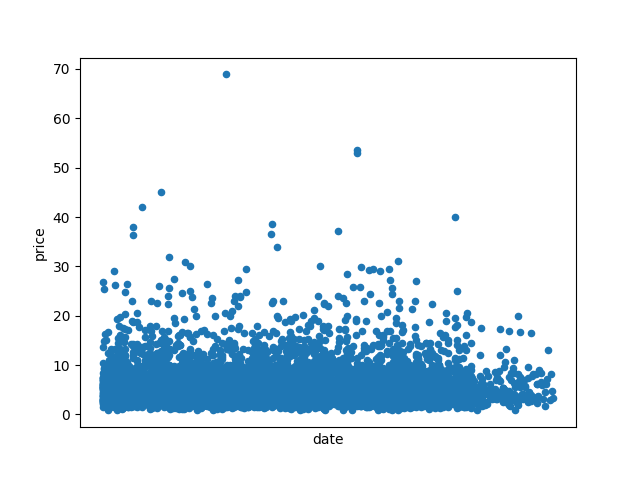
\includegraphics[width=0.45\textwidth, height=4cm]{price_vs_date} }\label{1a}}%
    \qquad
    \subfloat[\centering Plot of the housing price vs $date_{encoded}$]{{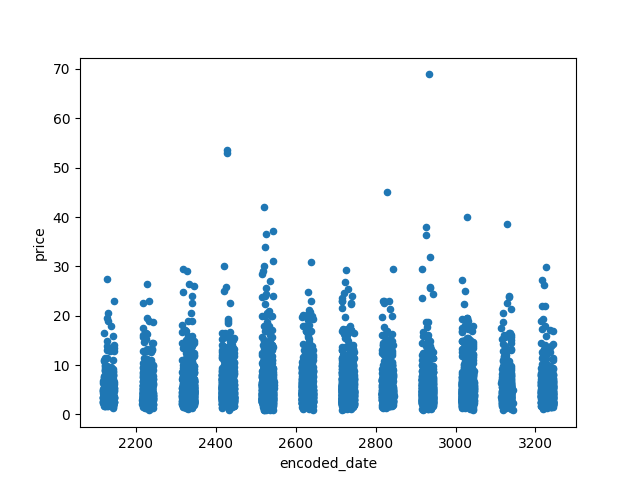
\includegraphics[width=0.45\textwidth, height=4cm]{price_vs_encoded_date} }\label{1b}}%
    \caption{Impact of encoding date on housing price prediction}%
    \label{fig:price}%
\end{figure}

Fig. \ref{1a} shows a scatter plot of the housing price vs the date. We see that there seems to be almost no correlation between the housing price and the date. However, using the encoded date, Fig. \ref{1b} shows a much more cleaner plot, with distinct changes in the encoded date values. So by knowing the value of the encoded date, we can predict the mean and variance of housing prices.\\ \\ \\ \\ \\ \\


\textbf{c.} Figures \ref{bed}, \ref{bath}, \ref{floor} show the variations in price with respect to each entitiy


\begin{figure}[h]
    \centering
    \subfloat[\centering Price vs No. of Bedrooms]{{\includegraphics[width=0.46\textwidth, height=4cm]{price_vs_bedrooms} }\label{bed}}%
    \qquad
    \subfloat[\centering Price vs No. of Bathrooms]{{\includegraphics[width=0.46\textwidth, height=4cm]{price_vs_bathrooms} }\label{bath}}%
    \qquad
    \subfloat[\centering Price vs No. of Floors]{{\includegraphics[width=0.46\textwidth, height=4cm]{price_vs_floors} }\label{floor}}%
    \caption{Variation of Price with: a. Bedrooms b. Bathrooms c. Floors}%
    \label{fig:price}%
\end{figure}

\pagebreak
\textbf{d.} The following two tables show the output Covariance (Table. 1) and Correlation (Table. 2) matrices. Fig. \ref{2d1}, \ref{2d2} show the scatter plots for sqft\_living15 vs sqft\_living and sqft\_lot15 vs sqft\_lot. Although we can conclude from the correlation matrix and the output plots that there is a lot of correlation between (sqft\_living15 and sqft\_living), and (sqft\_lot15 and sqft\_lot), they are not completely the same i.e the correlation is not $\pm1$. Therefore we can say that these features are not redundant.

\begin{table}[ht]
\centering
\begin{tabular}{ |p{2cm}||p{2cm}||p{2cm}|p{2cm}|p{2cm}|  }
 \hline
 \multicolumn{5}{|c|}{Covariance Matrix} \\
 \hline
  &	sqft-living&  sqft-lot&  sqft-living15&  sqft-lot15\\
 \hline
 sqft-living&	8.305303e+05&	6.473942e+06&	4.839029e+05&	4.836731e+06\\
 sqft-lot&	6.473942e+06&	1.697761e+09&	4.160910e+06&	8.924357e+08\\
 sqft-living15&	4.839029e+05&	4.160910e+06&	4.787260e+05&	3.568584e+06\\
 sqft-lot15&	4.836731e+06&	8.924357e+08&	3.568584e+06&	7.975678e+08\\
 \hline
\end{tabular}
\label{Tab:covar}
\end{table}


\begin{center}
\begin{table}[ht]
\begin{tabular}{ |p{2cm}||p{2cm}||p{2cm}|p{2cm}|p{2cm}|  }
 \hline
 \multicolumn{5}{|c|}{Correlation Matrix} \\
 \hline
  &	sqft-living&  sqft-lot&  sqft-living15&  sqft-lot15\\
 \hline
 sqft-living&	1.000000&	0.172406&	0.767427&	0.187928\\
 sqft-lot&	0.172406&	1.000000&	0.145951&	0.766928\\
 sqft-living15&	0.767427&	0.145951&	1.000000&	0.182629\\
 sqft-lot15&	0.187928&	0.766928&	0.182629&	1.000000\\
 \hline
\end{tabular}
\label{Tab:correl}
\end{table}
\end{center}

\begin{figure}[ht]
    \centering
    \subfloat[\centering Plot of sqft\_living15 vs sqft\_living]{{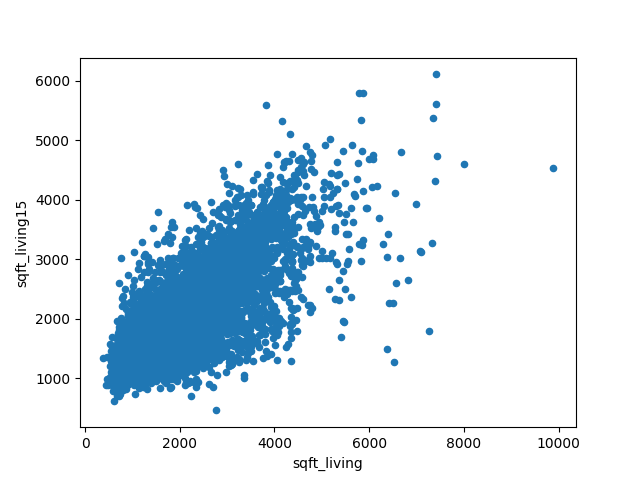
\includegraphics[width=0.45\textwidth, height=4cm]{sqft_living_15_vs_sqft_living} }\label{2d1}}%
    \qquad
    \subfloat[\centering Plot of sqft\_lot15 vs sqft\_lot]{{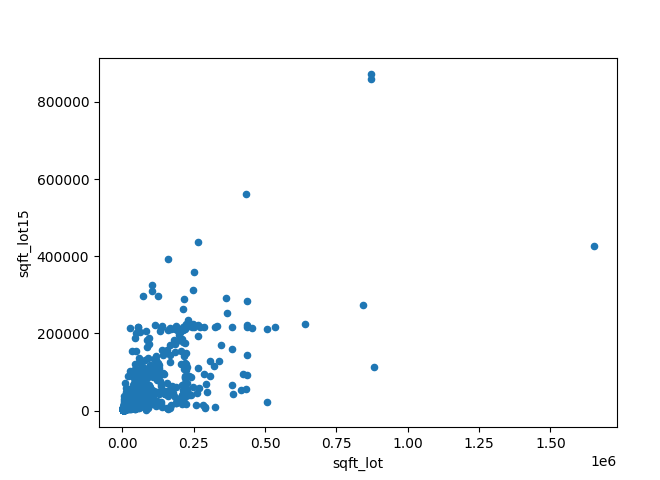
\includegraphics[width=0.45\textwidth, height=4cm]{sqft_lot_15_vs_sqft_lot} }\label{2d2}}%
    \caption{Scatter plots}%
    \label{fig:price}%
\end{figure}


\end{document}